% !TeX root = ../../Book4.tex
% 纲要标题：### 10.2 约化的线性和微分几何
% 纲要位置：几何学计划纲要.md，第 3857 行。
% 正文状态：初稿；尚未正式审核。

% 纲要内容开始
% 
% * 水平集的切空间
% * 辛正交与轨道方向
% * 闭二形式下降
% * 非退化性和商光滑性
% * Marsden–Weinstein 约化的完整证明
% 
% 纲要内容结束

\section{约化的线性和微分几何}
\label{g4:sec:1002}

固定矩映射的一个值，相当于给运动状态施加若干守恒量约束；再把对称群能够互相移动的状态视为相同，就得到约化空间。辛形式不能直接下降到任意轨道商：沿轨道改变切向量代表时，配对的值可能随之改变。本节将说明，矩映射水平集恰好使需要商掉的方向成为限制二形式的核。线性代数解决配对是否良定义，自由固有作用保证商是光滑流形，局部截面则把逐点配对组织成光滑闭形式。

\subsection{水平集的切空间}
\label{g4:subsec:1002:01}

沿用\cref{g4:def:1001:moment-map}的约定。有限维实 Lie 群 \(G\) 左作用于辛流形 \((M,\omega)\)，其 Lie 代数为 \(\mathfrak g\)，正向指数产生基本场 \(\xi_M\)。对矩映射 \(\mu:M\to\mathfrak g^*\)，记 \(\mu^\xi=\langle\mu,\xi\rangle\)，则
\[
	\mathrm{d}\mu^\xi=\iota_{\xi_M}\omega,
	\qquad
	\langle\mathrm{d}\mu_x(v),\xi\rangle=\omega_x(\xi_M(x),v).
\]
右侧同时记录了约束微分和轨道方向；这是约化证明中的基本等式。

\begin{proposition}\label{g4:prop:1002:moment-differential}
	设有限维实 Lie 群 \(G\) 辛作用于无边界辛流形 \((M,\omega)\)，且 \(\mu:M\to\mathfrak g^*\) 满足矩映射方程。令
	\[
		\rho_x:\mathfrak g\longrightarrow\mathrm{T}_xM,
		\quad \rho_x(\xi)=\xi_M(x),
		\qquad V_x=\operatorname{im}\rho_x,
		\quad\mathfrak g_x=\ker\rho_x.
	\]
	这里 \(V_x\) 是轨道切空间，\(\mathfrak g_x\) 是无穷小稳定子。则
	\begin{equation}\label{g4:eq:1002:moment-kernel-image}
		\ker\mathrm{d}\mu_x=V_x^\omega,
		\qquad
		\operatorname{im}\mathrm{d}\mu_x=\mathfrak g_x^\circ,
	\end{equation}
	其中 \(\mathfrak g_x^\circ\subset\mathfrak g^*\) 为消灭 \(\mathfrak g_x\) 的泛函空间。因此 \(x\) 是 \(\mu\) 的正则点，当且仅当 \(\mathfrak g_x=0\)。若 \(a\) 是正则值且 \(Z_a=\mu^{-1}(a)\ne\varnothing\)，则 \(Z_a\) 是余维 \(\dim G\) 的嵌入子流形，并且
	\begin{equation}\label{g4:eq:1002:level-tangent}
		\mathrm{T}_xZ_a=\ker\mathrm{d}\mu_x=V_x^\omega.
	\end{equation}
\end{proposition}
\begin{proof}
	对 \(v\in\mathrm{T}_xM\)，\(\mathrm{d}\mu_x(v)=0\) 等价于它与每个 \(\xi\in\mathfrak g\) 的配对为零，也就是 \(\omega_x(\xi_M(x),v)=0\) 对所有 \(\xi\) 成立。这给出第一个等式。

	把 \(\mathrm{d}\mu_x\) 转置，所得映射把 \(\xi\) 送到一形式 \(\omega_x(\rho_x\xi,\cdot)\)。辛形式的非退化性说明其核恰为 \(\mathfrak g_x\)，故 \(\mathrm{d}\mu_x\) 的秩等于 \(\dim\mathfrak g-\dim\mathfrak g_x\)。另一方面，若 \(\xi\in\mathfrak g_x\)，上面的配对恒为零，所以 \(\operatorname{im}\mathrm{d}\mu_x\subseteq\mathfrak g_x^\circ\)。两边维数相等，得到第二个等式和正则点判据。

	第一卷定理11.4.4的正则水平集定理给出最后的结论。具体说，在每个原像点附近，淹没标准形把 \(\mu-a\) 写成前 \(\dim G\) 个坐标的投影；令这些坐标为零就得到水平集，其切空间正是该投影的核。
\end{proof}

自由性蕴含 \(\mathfrak g_x=0\)。确实，若 \(\xi_M(x)=0\)，基本场积分曲线的唯一性说明 \(\exp(t\xi)x=x\) 对所有 \(t\) 成立；自由性迫使 \(\exp(t\xi)=e\)，在零时刻求导便得 \(\xi=0\)。反方向只能排除无穷小稳定子，不能排除离散的非平凡稳定子。

\begin{example}\label{g4:exm:1002:regular-not-free}
	在 \(\mathbb C\setminus\{0\}\) 上取 \(\omega=\mathrm{d}x\wedge\mathrm{d}y\)，令圆周按 \(e^{it}\cdot z=e^{ikt}z\) 作用，其中整数 \(k\ge2\)。基本场为 \(k(-y\partial_x+x\partial_y)\)，矩映射可取
	\[
		\mu(z)=-\frac{k}{2}|z|^2.
	\]
	其微分在这个空间处处非零，所以每个非空水平都是正则水平；但每一点的稳定子都有 \(k\) 个元素，作用并不自由。这个例子区分了水平集的光滑性与商映射所需的自由性。
\end{example}

\subsection{辛正交与轨道方向}
\label{g4:subsec:1002:02}

现在假设矩映射等变，即 \(\mu(gx)=\operatorname{Ad}_g^*\mu(x)\)，其中余伴随作用按前节的含 \(g^{-1}\) 约定定义。零在这个线性作用下固定，所以 \(Z=\mu^{-1}(0)\) 被整个 \(G\) 保持。于是每个基本场在 \(Z\) 上切向，轨道方向 \(V_x\) 包含于 \(\mathrm{T}_xZ\)。

\begin{proposition}\label{g4:prop:1002:zero-level-kernel}
	设有限维实 Lie 群 \(G\) 辛作用于无边界辛流形 \((M,\omega)\)，\(\mu:M\to\mathfrak g^*\) 是等变矩映射，\(0\) 是正则值且 \(Z=\mu^{-1}(0)\ne\varnothing\)。令 \(i:Z\hookrightarrow M\)，\(\beta=i^*\omega\)。则对每个 \(x\in Z\)，
	\begin{equation}\label{g4:eq:1002:zero-level-kernel}
		V_x\subseteq V_x^\omega=\mathrm{T}_xZ,
		\qquad
		(\mathrm{T}_xZ)^\omega=V_x,
		\qquad
		\ker\beta_x=V_x.
	\end{equation}
	特别地，轨道切空间各向同性，水平集切空间余各向同性。
\end{proposition}
\begin{proof}
	等变性给出 \(V_x\subseteq\mathrm{T}_xZ\)，而\cref{g4:prop:1002:moment-differential}给出 \(\mathrm{T}_xZ=V_x^\omega\)。\cref{g4:prop:0701:orthogonal-dimensions}的双重辛正交等式说明 \((\mathrm{T}_xZ)^\omega=(V_x^\omega)^\omega=V_x\)。限制型的核是
	\[
		\mathrm{T}_xZ\cap(\mathrm{T}_xZ)^\omega
		=\mathrm{T}_xZ\cap V_x=V_x,
	\]
	得到全部结论。
\end{proof}

也可直接检查轨道上的配对。由\cref{g4:prop:1001:equivariance-bracket}，
\[
	\omega_x(\xi_M(x),\eta_M(x))
	=\{\mu^\xi,\mu^\eta\}(x)
	=\langle\mu(x),[\xi,\eta]\rangle.
\]
它在零水平上为零。这个计算说明等变性怎样使群方向成为允许商掉的各向同性方向；而核的完整描述还需要上面的双重正交论证。

\ProseParagraphBreak

因此，每个 \(x\in Z\) 都给出一个辛向量空间
\[
	\mathrm{T}_xZ/V_x=V_x^\omega/V_x,
	\qquad
	\overline\omega_x([u],[v])=\omega_x(u,v).
\]
这是\cref{g4:thm:0701:linear-reduction}的逐点应用。下一步要确认：不同点得到的商空间能够成为同一个光滑商流形的切空间，而且这些配对随商点光滑变化。

\subsection{闭二形式下降}
\label{g4:subsec:1002:03}

先把形式下降的问题与辛非退化性分开。设 \(G\) 在流形 \(P\) 上自由且固有地作用，商映射记为 \(\pi:P\to B=P/G\)。第一卷定理17.2.6说明 \(B\) 是光滑流形，\(\pi\) 是满射淹没；第一卷引理17.2.5的局部乘积给出每点附近的光滑截面。截面选择一个轨道代表，但形式的值必须与这个选择无关。

\begin{definition}\label{g4:def:1002:basic-form}
	对有限维实 Lie 群 \(G\) 在无边界光滑流形 \(P\) 上的光滑作用，若微分形式 \(\alpha\) 满足 \(\iota_{\xi_P}\alpha=0\) 对所有 \(\xi\in\mathfrak g\) 成立，则称它为\term[shuipingxingshi]{水平形式}[horizontal form]。若它还对整个群不变，即 \(L_g^*\alpha=\alpha\) 对所有 \(g\in G\) 成立，则称它为\term[jibenxingshi]{基本形式}[basic form]。
\end{definition}

这里“水平”表示只要一个输入沿轨道，形式就为零，并没有为轨道方向选择一个补空间。水平性消除切向量提升的歧义；不变性消除轨道代表的歧义。

\begin{proposition}\label{g4:prop:1002:basic-descent}
	设有限维实 Lie 群 \(G\) 自由且固有地光滑作用于无边界流形 \(P\)，两者均为 Hausdorff、第二可数。赋予 \(B=P/G\) 自由固有商的光滑结构，并记商映射为 \(\pi\)。对 \(k\ge1\) 及 \(\alpha\in\Omega^k(P)\)，存在 \(\overline\alpha\in\Omega^k(B)\) 满足
	\begin{equation}\label{g4:eq:1002:basic-descent}
		\pi^*\overline\alpha=\alpha
	\end{equation}
	当且仅当 \(\alpha\) 为基本形式；存在时 \(\overline\alpha\) 唯一。并且 \(\overline\alpha\) 闭当且仅当 \(\alpha\) 闭。
\end{proposition}
\begin{proof}
	若 \(\alpha=\pi^*\overline\alpha\)，则 \(\pi\circ L_g=\pi\) 给出不变性，而 \(\mathrm{d}\pi(\xi_P)=0\) 给出水平性。

	反过来，给定 \(b\in B\) 与 \(u_1,\ldots,u_k\in\mathrm{T}_bB\)，选择 \(x\in\pi^{-1}(b)\)，并借淹没性取 \(v_j\in\mathrm{T}_xP\)，使 \(\mathrm{d}\pi_x(v_j)=u_j\)。定义
	\[
		\overline\alpha_b(u_1,\ldots,u_k)
		=\alpha_x(v_1,\ldots,v_k).
	\]
	局部乘积中 \(\pi\) 是忘掉群因子的投影，因此 \(\ker\mathrm{d}\pi_x\) 正是基本场值张成的轨道切空间。改变任一提升只增加一个这样的向量，水平性使右侧不变。若改取另一代表 \(x'=gx\)，可用 \(\mathrm{d}L_g(v_j)\) 作提升；群不变性又使右侧不变。这证明定义良好，并给出拉回等式。

	取任一光滑局部截面 \(s:U\to P\)，则这个逐点定义在 \(U\) 上恰为 \(s^*\alpha\)，所以光滑。不同截面的拉回一致，已经由刚才的代表与提升无关性保证，因而这些局部形式粘成整体形式。任何满足拉回等式的形式都必须在 \(U\) 上等于 \(s^*\alpha\)，所以唯一。

	同样的局部截面说明 \(\pi^*\) 在所有次数上单射：若 \(\pi^*\gamma=0\)，则 \(\gamma|_U=s^*\pi^*\gamma=0\)。拉回与外微分交换，故
	\[
		\pi^*\mathrm{d}\overline\alpha
		=\mathrm{d}\pi^*\overline\alpha
		=\mathrm{d}\alpha.
	\]
	单射性给出两个闭性条件的等价。
\end{proof}

这条判据要求整个群的不变性。若 \(G\) 连通，闭形式的水平性通过 Cartan 公式给出 \(\mathcal L_{\xi_P}\alpha=0\)，沿基本场流积分并用第一卷命题16.2.5的指数生成性，可得到群不变性；若群不连通，仅有无穷小不变性不能控制其他连通分支。

\begin{example}\label{g4:exm:1002:descent-conditions}
	对 \(\mathbb R\) 在 \(\mathbb R_t\times\mathbb R_x\times\mathbb R_y\) 上沿 \(t\) 的平移，形式 \(\mathrm{d}t\wedge\mathrm{d}x\) 闭且不变，却不水平，因为插入 \(\partial_t\) 得到 \(\mathrm{d}x\)。所以它不下降到 \((x,y)\) 平面。

	再令离散群 \(\mathbb Z\) 在 \(\mathbb R^2\) 上按 \(m\cdot(x,y)=(x+m,y)\) 作用。这个作用自由且固有；由于群的 Lie 代数为零，每个形式都满足水平条件。但闭形式 \(e^x\mathrm{d}x\wedge\mathrm{d}y\) 在平移一次后乘以 \(e\)，因此不下降到圆柱 \((\mathbb R/\mathbb Z)\times\mathbb R\)。
\end{example}

\subsection{非退化性和商光滑性}
\label{g4:subsec:1002:04}

固有性的定义约束映射 \((g,x)\mapsto(gx,x)\)：若出发点和到达点都限制在紧集内，群参数也不能逃逸。自由固有商定理的证明正是先用逆函数定理找到横截面，再用这个条件排除远处群元素把横截面送回自身。局部乘积 \(G\times S\cong GS\) 随后提供商坐标和截面。不同轨道的分离性来自轨道等价关系闭；商投影是开映射，故源的可数基给出商的可数基。这些步骤保证商满足 Hausdorff 性与第二可数性，既有局部坐标也有正确的整体拓扑。

\ProseParagraphBreak

现在设 \(\beta\) 已经下降。商上的形式可能仍退化：水平性只说明轨道方向包含在 \(\ker\beta\) 中，只有当它们恰为全部核时，取商才能消除所有退化方向。

\begin{proposition}\label{g4:prop:1002:quotient-nondegeneracy}
	设有限维实 Lie 群 \(G\) 自由且固有地光滑作用于无边界流形 \(P\)，两者均为 Hausdorff、第二可数。设 \(\beta\) 为 \(P\) 上的基本闭二形式，\(\overline\beta\) 是它在 \(B=P/G\) 上的下降形式。则
	\begin{equation}\label{g4:eq:1002:quotient-tangent}
		\mathrm{T}_{[x]}B\cong
		\mathrm{T}_xP/\mathrm{T}_x(Gx),
		\qquad
		\ker\overline\beta_{[x]}
		\cong\ker\beta_x/\mathrm{T}_x(Gx).
	\end{equation}
	因此 \(\overline\beta\) 是辛形式，当且仅当 \(\ker\beta_x=\mathrm{T}_x(Gx)\) 对每个 \(x\in P\) 成立。
\end{proposition}
\begin{proof}
	第一卷定理17.2.6给出商流形与满射淹没 \(\pi\)。在局部乘积坐标中，\(\mathrm{d}\pi_x\) 忘掉群方向，所以其核是 \(\mathrm{T}_x(Gx)\)；线性同态定理给出第一项同构。

	若 \(u=\mathrm{d}\pi_x(v)\)，则 \(u\) 与全部商切向量的 \(\overline\beta\) 配对为零，当且仅当 \(\beta_x(v,w)=0\) 对全部 \(w\in\mathrm{T}_xP\) 成立，因为 \(\mathrm{d}\pi_x\) 满射。这等价于 \(v\in\ker\beta_x\)。水平性又保证 \(\mathrm{T}_x(Gx)\subseteq\ker\beta_x\)，从而得到第二项同构。闭性已由\cref{g4:prop:1002:basic-descent}证明，故核为零恰好是辛条件。
\end{proof}

这里没有假定群紧。若 \(G\) 紧，则作用自动固有：给定 \(P\times P\) 中紧集 \(C\)，其第二投影为紧集 \(K\)，\(C\) 在作用映射 \((g,x)\mapsto(gx,x)\) 下的原像是 \(G\times K\) 的闭子集，所以紧。非紧群则须实际检查固有性，不能从自由性推断。

\subsection{Marsden–Weinstein 约化的完整证明}
\label{g4:subsec:1002:05}

把水平集上的核计算与形式下降合在一起，就得到\term[MarsdenWeinsteinyuehuadingli]{Marsden--Weinstein 约化定理}[Marsden--Weinstein reduction theorem]。\footnote{Jerrold Eldon Marsden（1942--2010），加拿大出生、长期在美国工作的数学家，研究几何力学、辛约化与动力系统。}下面先处理零值；它对整个余伴随作用固定，所以全部群方向都留在同一个水平集内。

\begin{theorem}[Marsden--Weinstein 约化]\label{g4:thm:1002:symplectic-reduction}
	设 \(G\) 为 \(r\) 维实 Lie 群，\((M^{2n},\omega)\) 为无边界辛流形，二者均为 Hausdorff、第二可数。设 \(G\) 在 \(M\) 上光滑辛作用，且有等变矩映射 \(\mu:M\to\mathfrak g^*\)。假设 \(0\) 是正则值，\(Z=\mu^{-1}(0)\ne\varnothing\)，并且 \(G\) 在 \(Z\) 上的限制作用自由且固有。则
	\[
		M_{\mathrm{red}}=Z/G
	\]
	在商拓扑下是 \(2n-2r\) 维无边界光滑流形，商映射 \(\pi:Z\to M_{\mathrm{red}}\) 是满射淹没。存在唯一辛形式 \(\omega_{\mathrm{red}}\) 使
	\begin{equation}\label{g4:eq:1002:reduction-pullback}
		\pi^*\omega_{\mathrm{red}}=i^*\omega,
		\qquad i:Z\hookrightarrow M.
	\end{equation}
	逐点地，\(\mathrm{T}_{[x]}M_{\mathrm{red}}\) 与 \(V_x^\omega/V_x\) 辛同构。
\end{theorem}
\begin{proof}
	正则水平集定理使 \(Z\) 成为 \(2n-r\) 维嵌入子流形。等变性使 \(Z\) 对 \(G\) 不变，因此题设的限制作用有定义。自由固有商定理给出 \(Z/G\) 的光滑结构和满射淹没 \(\pi\)，维数再减去 \(r\)，得到 \(2n-2r\)。

	令 \(\beta=i^*\omega\)。因为作用保辛且 \(Z\) 不变，\(\beta\) 对整个 \(G\) 不变。对 \(x\in Z\)、\(v\in\mathrm{T}_xZ\)，矩映射方程给出
	\[
		\beta_x(\xi_M(x),v)
		=\omega_x(\xi_M(x),v)
		=\mathrm{d}\mu^\xi_x(v)=0,
	\]
	所以 \(\beta\) 水平；\(\mathrm{d}\beta=i^*\mathrm{d}\omega=0\)，所以它闭。\cref{g4:prop:1002:basic-descent}于是给出唯一光滑闭二形式 \(\omega_{\mathrm{red}}\)，满足所需拉回等式。

	由\cref{g4:prop:1002:zero-level-kernel}，\(\ker\beta_x=V_x\)，而自由作用下 \(V_x=\mathrm{T}_x(Gx)=\ker\mathrm{d}\pi_x\)。\cref{g4:prop:1002:quotient-nondegeneracy}遂给出 \(\omega_{\mathrm{red}}\) 非退化。最后，\(\mathrm{T}_xZ=V_x^\omega\) 和拉回等式说明商切空间上的配对恰为 \([u],[v]\mapsto\omega_x(u,v)\)，就是线性约化的辛同构。
\end{proof}

称 \((M_{\mathrm{red}},\omega_{\mathrm{red}})\) 为在零值处的\term[xinyuehuakongjian]{辛约化空间}[symplectic reduced space]，也称辛商。若作用在水平集上自由，\cref{g4:prop:1002:moment-differential}已经保证零是正则值；定理仍将正则性列出，以明确水平集与商流形两个构造分别使用的条件。紧群版本及线性证明可对照 Cannas da Silva 的定理6.1、引理6.3--6.4与命题6.5。这里用第一卷的自由固有商定理处理非紧群。\cite[第6.1节，第160--163页]{Cannas2006Symplectic}

% !TeX root = ../Book4.tex
\begin{figure}[htbp]
	\centering
	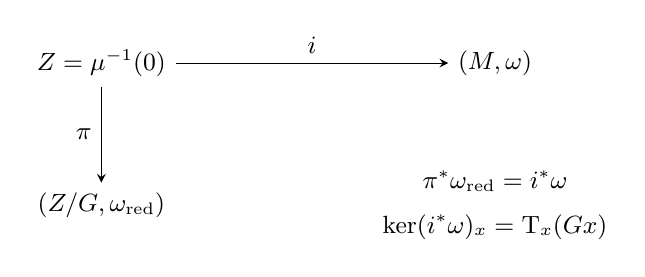
\begin{tikzpicture}[font=\small,>=stealth]
		\node (Z) at (0,1.5) {\(Z=\mu^{-1}(0)\)};
		\node (M) at (5,1.5) {\((M,\omega)\)};
		\node (B) at (0,-0.3) {\((Z/G,\omega_{\mathrm{red}})\)};
		\draw[->] (Z)--node[above] {\(i\)} (M);
		\draw[->] (Z)--node[left] {\(\pi\)} (B);
		\node[align=center] at (5,-0.3) {\(\pi^*\omega_{\mathrm{red}}=i^*\omega\)\\[5pt]\(\ker(i^*\omega)_x=\mathrm{T}_x(Gx)\)};
	\end{tikzpicture}
	\caption[水平集与轨道商]{先把辛形式限制到矩映射的零水平，再沿群轨道取商。限制型的核恰为商映射消去的方向，所以商上的形式非退化。}
	\label{g4:fig:1002:reduction-diagram}
\end{figure}


\begin{example}\label{g4:exm:1002:translation-reduction}
	在 \(\mathbb R^{2n}_{q,p}\) 中，让 \(G=\mathbb R^r\)、\(r\le n\)，平移前 \(r\) 个位置坐标。作用自由。按第一卷命题17.2.2的序列判据，它也固有：若 \(x_j\to x\)、\(t_jx_j\to y\)，群参数 \(t_j\) 等于两个点前 \(r\) 个位置坐标的差，因而收敛。矩映射为 \(\mu=(p_1,\ldots,p_r)\)，所以
	\[
		Z=\{p_1=\cdots=p_r=0\},\qquad
		Z/G\cong\mathbb R^{2(n-r)}.
	\]
	商映射保留 \((q^{r+1},\ldots,q^n,p_{r+1},\ldots,p_n)\)，约化形式为
	\[
		\omega_{\mathrm{red}}=\sum_{j=r+1}^n\mathrm{d}q^j\wedge\mathrm{d}p_j.
	\]
	水平约束先去掉 \(r\) 个动量方向，轨道商再去掉与之配对的 \(r\) 个位置方向。\(r=n\) 时约化空间为一点，其零二形式在零维切空间上非退化。
\end{example}

非零值的差别在于水平集未必被整个群保持。对 \(a\in\mathfrak g^*\)，定义余伴随稳定子
\[
	G_a=\{g\in G:\operatorname{Ad}_g^*a=a\}.
\]
它是闭子群，第一卷定理16.3.6赋予它嵌入 Lie 子群结构。其 Lie 代数为
\begin{equation}\label{g4:eq:1002:coadjoint-stabilizer-algebra}
	\mathfrak g_a=\{\xi\in\mathfrak g:
	\langle a,[\eta,\xi]\rangle=0\text{ 对所有 }\eta\in\mathfrak g\}.
\end{equation}
确实，\(\left.\frac{\mathrm{d}}{\mathrm{d}t}\right|_0\operatorname{Ad}_{\exp(t\xi)}^*a\) 与 \(\eta\) 的配对是 \(-\langle a,[\xi,\eta]\rangle\)。这个导数为零时，表示的单参数群规律使整个曲线的导数为零，因此 \(\exp(t\xi)\) 对所有 \(t\) 固定 \(a\)；反向由求导得到。闭子群定理中的指数判据便给出所列 Lie 代数。

\begin{theorem}\label{g4:thm:1002:nonzero-reduction}
	设 \(G\) 为有限维实 Lie 群，\((M^{2n},\omega)\) 为无边界辛流形，二者均为 Hausdorff、第二可数。设 \(G\) 辛作用于 \(M\)，\(\mu:M\to\mathfrak g^*\) 为等变矩映射。若 \(a\) 为正则值、\(Z_a=\mu^{-1}(a)\ne\varnothing\)，并且 \(G_a\) 在 \(Z_a\) 上自由且固有地作用，则
	\[
		M_a=Z_a/G_a
	\]
	是维数 \(2n-\dim G-\dim G_a\) 的无边界光滑流形，并有唯一辛形式 \(\omega_a\) 满足
	\begin{equation}\label{g4:eq:1002:nonzero-reduction}
		\pi_a^*\omega_a=i_a^*\omega,
		\qquad
		\ker(i_a^*\omega)_x=\{\xi_M(x):\xi\in\mathfrak g_a\}.
	\end{equation}
	这里 \(i_a:Z_a\hookrightarrow M\)、\(\pi_a:Z_a\to M_a\) 分别为包含映射与商映射。
\end{theorem}
\begin{proof}
	等变性说明 \(G_a\) 保持 \(Z_a\)，正则性给出其维数为 \(2n-\dim G\)。仍记 \(V_x=\{\xi_M(x):\xi\in\mathfrak g\}\)，则
	\[
		\mathrm{T}_xZ_a=V_x^\omega,
		\qquad
		\ker(i_a^*\omega)_x=V_x^\omega\cap V_x.
	\]
	这里的 \(V_x\) 使用整个 \(\mathfrak g\)，不能先把它换成 \(\mathfrak g_a\)。对于其中的向量 \(\xi_M(x)\)，有
	\[
		\langle\mathrm{d}\mu_x(\xi_M(x)),\eta\rangle
		=\omega_x(\eta_M(x),\xi_M(x))
		=\langle a,[\eta,\xi]\rangle.
	\]
	因此 \(\xi_M(x)\in\mathrm{T}_xZ_a\) 当且仅当 \(\xi\in\mathfrak g_a\)，这恰好识别出限制型的全部核。

	\(i_a^*\omega\) 对 \(G_a\) 不变，且对其轨道方向水平。自由固有商定理赋予 \(Z_a/G_a\) 光滑结构，维数减去 \(\dim G_a\)。\cref{g4:prop:1002:basic-descent}给出唯一闭下降形式，而刚才的核等式及\cref{g4:prop:1002:quotient-nondegeneracy}证明它非退化。
\end{proof}

若整个 \(G\) 在 \(M\) 上的作用自由且固有，上述限制条件自动成立。自由性直接继承；对于固有性，\(G_a\) 与 \(Z_a\) 都闭，限制作用映射在紧集上的原像是原作用相应紧原像的闭子集。因此通常可以从环境作用的固有性得到所需条件，但定理只要求水平集上的限制作用固有。

\ProseParagraphBreak

当 \(a\) 被整个余伴随作用固定时，\(G_a=G\)，且 \(\mu-a\) 仍等变，非零值约化就是平移矩映射后的零值约化。一般 \(a\) 虽然也可从 \(\mu\) 中减去，却会使等变性改变：\((\mu-a)(gx)-\operatorname{Ad}_g^*(\mu-a)(x)=\operatorname{Ad}_g^*a-a\)。所以不能不检查这一项，就将任意非零值当作零值。稳定子版本同时说明，非零值处要商掉的是 \(G_a\) 的轨道方向，而不是全部 \(G\) 方向。
% 纲要条目排为编号小节标题，并进入目录与书签；说明段仍保留于纲要注释中。
